\section{Parameter Estimation}
\label{sec:parameter-estimation}

We have learned a few elementary ways to determine the \textit{family of distributions}. Now, we learn how to \textit{estimate parameters of distributions}. As a result, a large family will be reduced to just one distribution that we can use for performance evaluation, forecasting, etc.

Statisticians developed a number of estimation techniques, each having certain optimal properties. Two rather popular methods are discussed in this section:
\begin{itemize}
  \item method of moments, and
  \item method of maximum likelihood.
\end{itemize}

\subsection{Method of Moments}
\label{subsec:method-of-moments}

\subsubsection{Moments}
\label{subsubsec:moments}

First, let us define the moments.
\begin{definition}{}
  The $k$-th \textbf{population moment} is defined as
  \begin{equation*}
    \mu_k = \expck{X}{k}
  \end{equation*}
  The $k$-th \textbf{sample moment}
  \begin{equation*}
    m_k = \frac{1}{n} \sum_{i=1}^{n} X_i^k
  \end{equation*}
  estimates $\mu_k$ from a sample $(X_1,\ \ldots,\ X_n)$. \\

  The first sample moment is the sample mean $\bar{X}$.  
\end{definition}

Central moments are computed similarly, after centralizing the data, that is, subtracting the mean.

\begin{definition}{}
  For $k \geq 2$, the $k$-th \textbf{population central moment} is defined as
  \begin{equation*}
    \mu_k' = \expck{(X - \mu_1)}{k}
  \end{equation*}
  The $k$-th \textbf{sample central moment}
  \begin{equation*}
    m_k' = \frac{1}{n} \sum_{i=1}^{n} (X_i - \bar{X})^k
  \end{equation*}
  estimates $\mu_k$ from a sample $(X_1,\ \ldots,\ X_n)$.
\end{definition}

\textbf{Remark:} 
\begin{itemize}
  \item The \textit{second population central moment is variance} $\var{X}$.
  \item The \textit{second sample central moment is sample variance}, although $(n - 1)$ in its denominator is now replaced by $n$.
\end{itemize}
We mentioned that estimation methods are not unique. For unbiased estimation of $\sigma^2 = \var{X}$, we use
\begin{equation*}
  s^2 = \frac{1}{n - 1} \sum_{i=1}^{n} (X_i - \bar{X})^2
\end{equation*}
however, method of moments and method of maximum likelihood produce a different version,
\begin{equation*}
  S^2 = m_2' = \frac{1}{n} \sum_{i=1}^{n} (X_i - \bar{X})^2
\end{equation*}


\subsubsection{Estimation}
\label{subsubsec:estimation}

\textbf{Method of moments} is based on a simple idea. Since our sample comes from a family of distributions $\{ F(\theta) \}$, we choose such a member of this family whose properties are close to properties of our data. Namely, we shall \textit{match the moments}.

To estimate $k$ parameters, equate the first $k$ population and sample moments,
\begin{equation*}
  \begin{cases}
    \mu_1 = m_1 \\
    \cdots\ \cdots\ \cdots \\
    \mu_k = m_k \\
  \end{cases}
\end{equation*}
The left-hand sides of these equations depend on the distribution parameters. The right-hand sides can be computed from data. The \textbf{method of moments estimator} is the solution of this system of equation.

\begin{example}{ (Poisson)}
  To estimate parameter $\lambda$ of Poisson($\lambda$) distribution, we recall that
  \begin{equation*}
    \mu_1 = \expc{X} = \lambda
  \end{equation*}
  There is only one unknown parameter, hence we write one equation,
  \begin{equation*}
    \mu_1 = \lambda = m_1 = \bar{X}
  \end{equation*}
  ``Solving'' it for $\lambda$, we obtain
  \begin{equation*}
    \hat{\lambda} = \bar{X}
  \end{equation*}
  the method of moments estimator of $\lambda$.
\end{example}

\textbf{\textit{Check the examples 9.4 and 9.5 from textbook.}}

\noindent On rare occasions, when $k$ equations are not enough to estimate $k$ parameters, we'll consider higher moments.

\vspace*{\fill}
\columnbreak

\begin{example}{ (Normal)}
  Suppose we already know the mean $\mu$ of a Normal distribution and would like to estimate the variance $\sigma^2$. Only one parameter $\sigma^2$ is unknown; however, the first method of moments equation
  \begin{equation*}
    \mu_1 = m_1
  \end{equation*}
  does not contain $\sigma^2$ and therefore does not produce its estimate. We then consider the second equation, say,
  \begin{equation*}
    \mu_2' = \sigma^2 = m_2' = S^2
  \end{equation*}
  which gives us the method of moments estimate immediately, $\hat{\sigma}^2 = S^2$.
\end{example}

Method of moments estimates are typically easy to compute. They can serve as a quick tool for estimating parameters of interest.


\subsection{Method of Maximum Likelihood}
\label{subsec:method-of-maximum-likelihood}

Since the sample $\boldsymbol{X} = (X_1,\ \ldots,\ X_n)$ has already been observed, we find such parameters that maximize the probability (likelihood) for this to happen. In other words, we make the event that has already happened to be as likely as possible. This is yet another way to make the chosen distribution consistent with the observed data.
\begin{definition}{}
  \textbf{Maximum likelihood estimator} is the parameter value that maximizes the likelihood of the observed sample.
  \begin{itemize}
    \item For a discrete distribution, we maximize the joint pmf of data $P(X_1,\ \ldots,\ X_n)$.
    \item For a continuous distribution, we maximize the joint density $f(X_1,\ \ldots,\ X_n)$.
  \end{itemize}
\end{definition}

\subsubsection{Discrete Case}
\label{subsubsec:disc-case}

For a discrete distribution, the probability of a given sample is the joint pmf of data,
\begin{align*}
  \prob{\boldsymbol{X} = (X_1,\ \ldots,\ X_n)} = P(\boldsymbol{X}) &= P(X_1,\ \ldots,\ X_n) \\
  &= \prod_{i=1}^{n} P(X_i)
\end{align*}
because in a simple random sample, all observed $X_i$ are independent.

To maximize this likelihood, we consider the critical points by taking derivatives with respect to all unknown parameters and equating them to 0.  The maximum can only be attained at such parameter values $\theta$ where the derivative $\frac{\partial}{\partial\theta} P(X)$ equals 0, where it does not exist, or at the boundary of the set of possible values of $\theta$.

A nice computational shortcut is to take logarithms first. Differentiating the sum
\begin{equation*}
  \ln \prod_{i=1}^{n} P(X_i) = \sum_{i=1}^{n} \ln P(X_i)
\end{equation*}
is easier than differentiating the product $\prod P(X_i)$. Besides, logarithm is an increasing function, so the likelihood $P(\boldsymbol{X})$ and the log-likelihood $\ln P(\boldsymbol{X})$ are maximized by exactly the same parameters.

\textbf{\textit{Check the example 9.7 from textbook.}}

\subsubsection{Continuous Case}
\label{subsubsec:cont-case}

In the continuous case, the probability to observe exactly the given number $X = x$ is $0$. Instead, the method of maximum likelihood will maximize the
probability of observing ``almost'' the same number.

For a very small $h$,
\begin{equation*}
  \prob{x - h < X < x + h} = \int_{x - h}^{x + h} f(y) d(y) \approx (2h) f(x)
\end{equation*}
That is, the probability of observing a value close to $x$ is proportional to the density $f(x)$ (see Figure 1). Then, for a sample $\bs{X} = (X_1,\ \ldots,\ X_n)$, the maximum likelihood method will maximize the joint density $f(X_1,\ \ldots,\ X_n)$.
\begin{figure}[H]
  \centering
  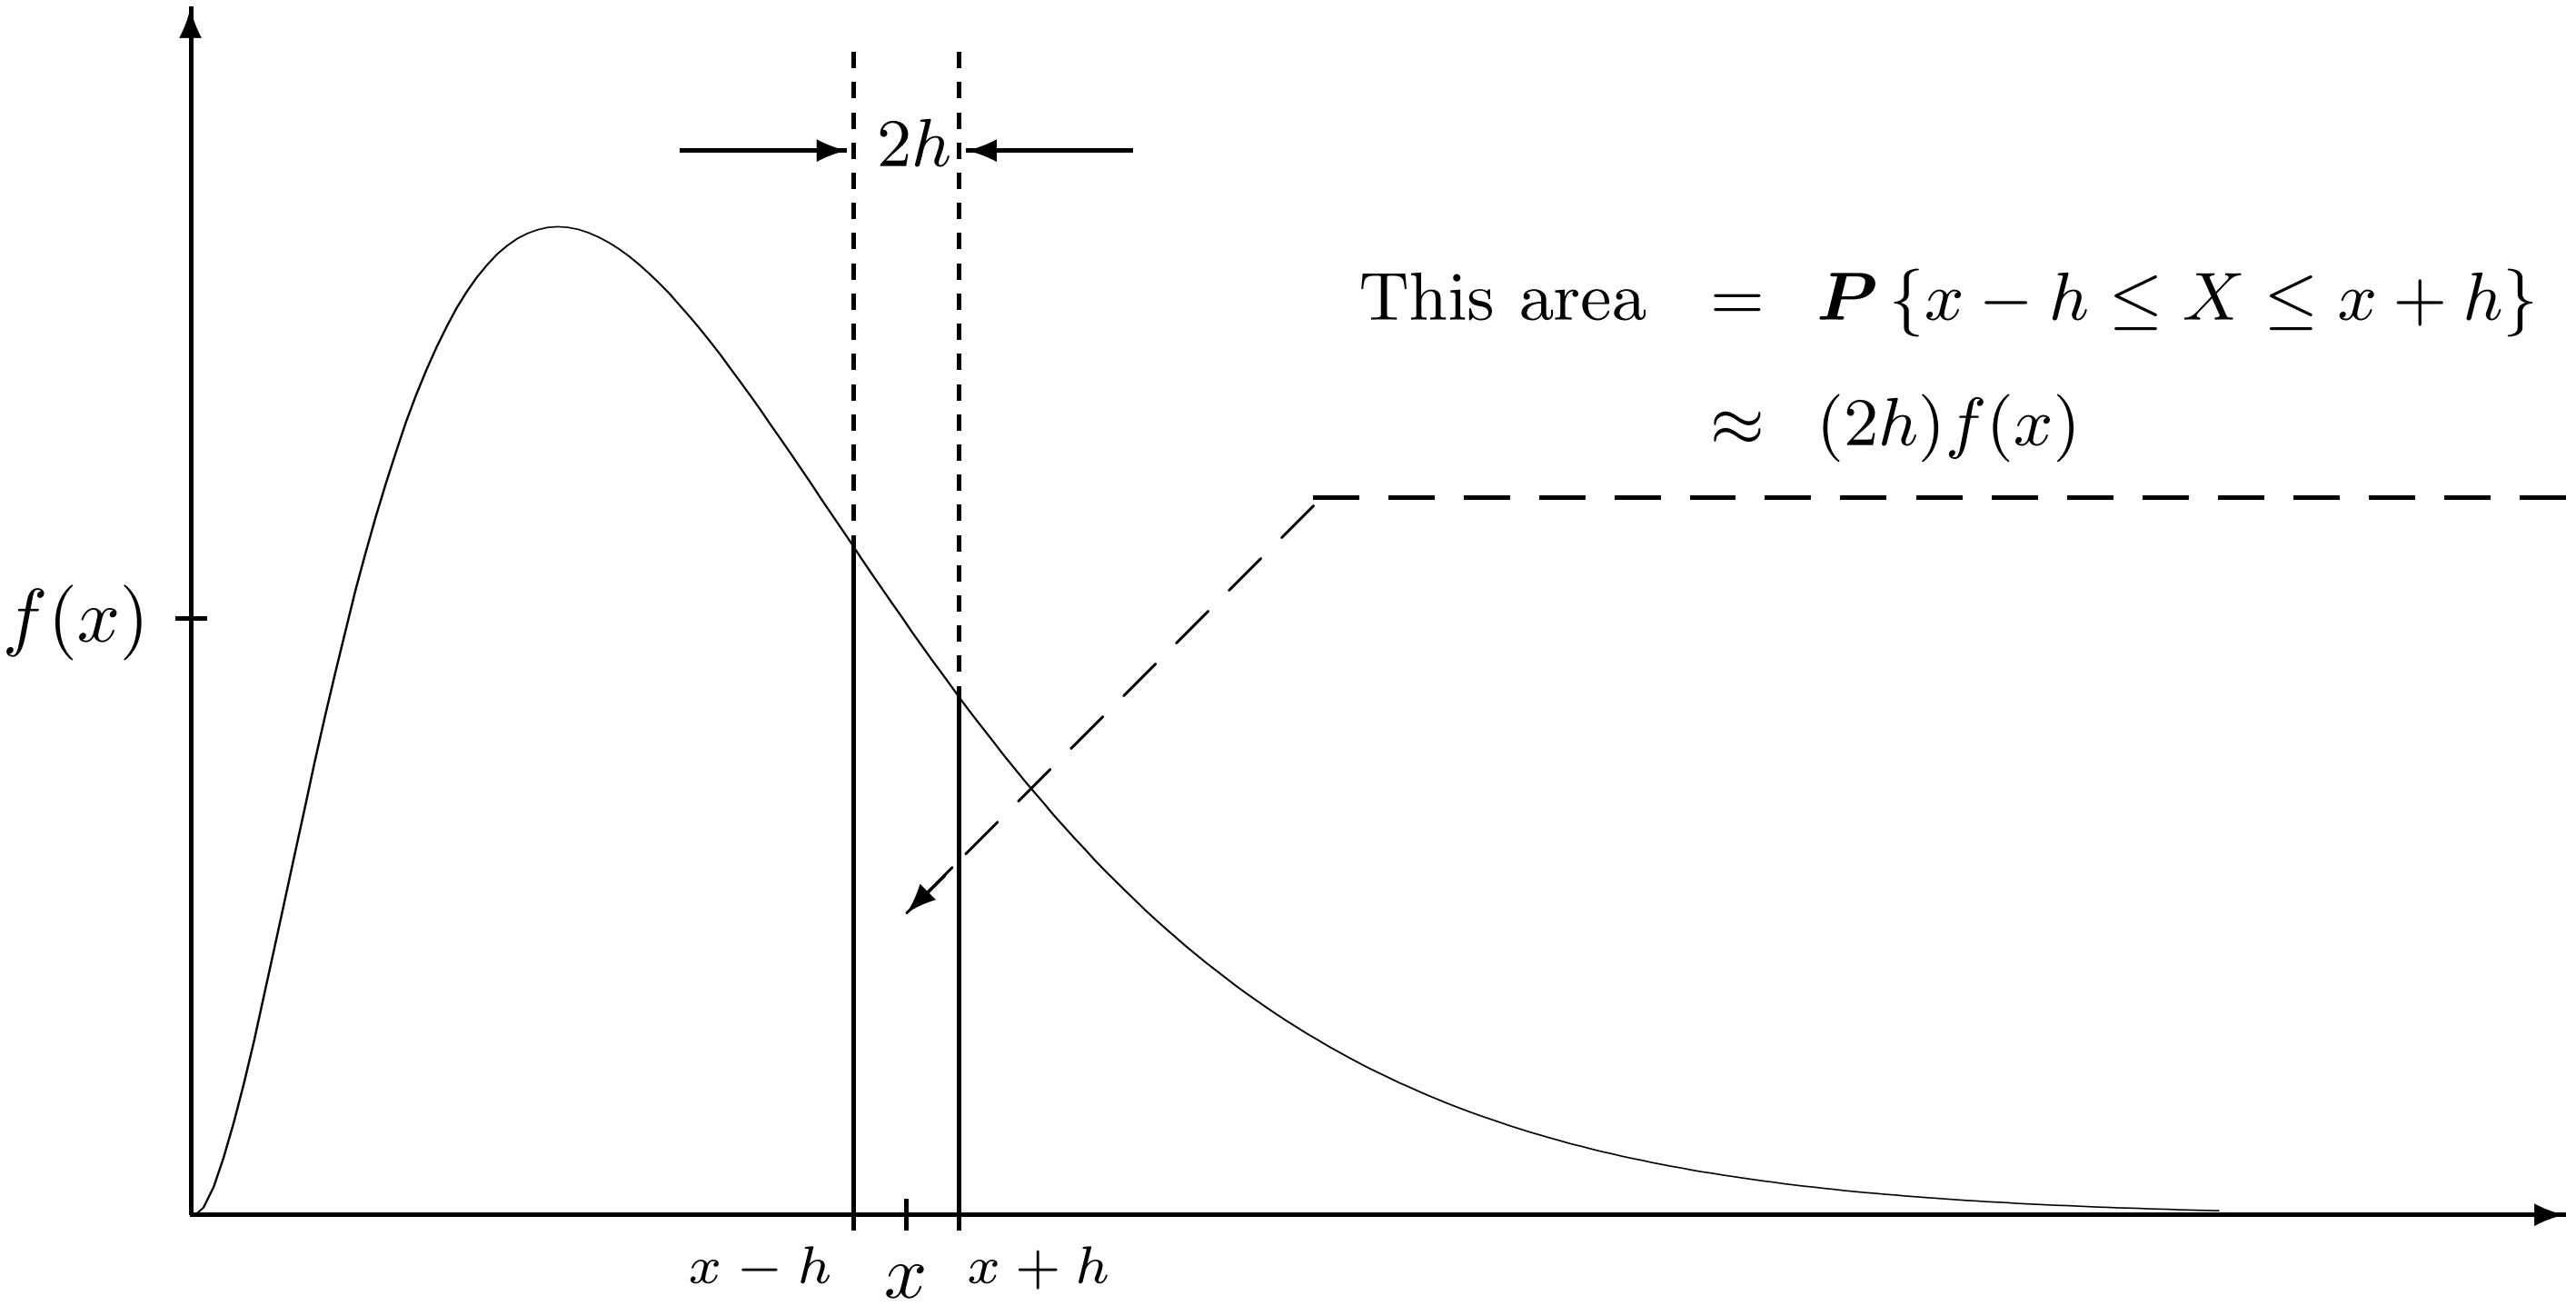
\includegraphics[width=\linewidth]{img/fig-9.1.png}
  \caption{}
  \label{fig:9.1}
\end{figure}

\textbf{\textit{Check the examples 9.8 and 9.9 from textbook.}}

Sometimes the likelihood has no critical points inside its domain, then it is maximized at the boundary.

When we estimate more than $1$ parameter, all the partial derivatives should be equal $0$ at the critical point. If no critical points exist, the likelihood is again maximized on the boundary.

Maximum likelihood estimators are rather popular because of their nice properties. Under mild conditions, these estimators are consistent, and for large samples, they have an approximately Normal distribution. Often in complicated problems, finding a good estimation scheme may be challenging whereas the maximum likelihood method always gives a reasonable solution.

\vspace*{\fill}
\columnbreak


\subsection{Estimation of Standard Errors}
\label{subsec:estimation-of-standard-errors}

Standard errors can serve as measures of their accuracy. To estimate them, we derive an expression for the standard error and estimate all the unknown parameters in it.

\begin{example}{ (Estimation of the Poisson Parameter)}
  By the method of moments and maximum likelihood estimators of the Poisson parameter $\lambda$ is $\hat{\lambda} = \bar{X}$. Let us now estimate the
  standard error of $\hat{\lambda}$.

  \textbf{Solution:}
  There are at least two ways to do it.

  On one hand, $\sigma = \sqrt{\lambda}$ for the Poisson($\lambda$) distribution, so $\sigma(\hat{\lambda}) = \sigma(\bar{X}) = \sigma / \sqrt{n} = \sqrt{\lambda / n}$, as we know before (\textit{textbook (8.2) on p. 213}). Estimating $\lambda$ by $\bar{X}$, we obtain
  \begin{equation*}
    s_1(\hat{\lambda}) = \sqrt{\frac{\bar{X}}{n}} = \frac{\sqrt{\Sigma X_i}}{n}
  \end{equation*}

  On the other hand, we can use the sample standard deviation and estimate the standard error of the sample mean,
  \begin{equation*}
    s_2(\hat{\lambda}) = \frac{s}{\sqrt{n}} = \sqrt{\frac{\Sigma (X_i - \bar{X})^2}{n (n-1)}}
  \end{equation*}
  Apparently, we can estimate the standard error of $\hat{\lambda}$ by two good estimators, $s_1$ and $s_2$.
\end{example}

